
\chapter{机械能}\minitoc[n]
\section{教学要求}
通过本章的学习,要使学生认识到:各种形式的能可以
相互转化,而且在转化过程中保持守恒;功是能的转化的
量度.

能的转化和守恒,是贯穿全部物理学的基本规律之一.解
决力学问题,从能量的观点人手分析,往往是很方便的.因此,
在本章的教学中,要特别注意培养学生从能量的观点来分析
问题.

这一章的教学要求是:
\begin{enumerate}
\item 理解功的概念,掌握功的计算公式,了解正负功的
意义.
\item 理解功率的概念,掌握功率的公式$P=Fv$.
\item 理解动能的概念,掌握动能的公式,掌握动能定理,会
运用动能定理解决力学问题.
\item 理解重力势能的概念,掌握重力势能的公式,掌握重
力做功与重力势能变化的关系.了解重力做功与路径无关是
引入重力势能的前提.
\item 了解弹性势能的概念,知道弹力做功与弹性势能
方关.
\item 掌握机械能守恒定律,会运用这个定律解决力学
问题.
\item 理解功和能的关系,知道功是能的转化的量度,学习
用能的观点来分析决力学问题.
\end{enumerate}


下面对这一章的教学内容作些具体说明.

为了给讲解动能和重力势能做好准备,教材安排了“能
量”一节,让学生对什么是能量以及功和能的关系有一个概括
的了解.什么是能量?许多课本中常常引用的“能是物体做功
的本领”,这个定义,严格说来有些不妥.从状态函数的角度
给出能量的普遍定义,中学生又难于接受 因此,教材沿用初
中物理的提法:一个物体能够做功,就说这个物体具有能量.
这并不是给能量下定义,只是使学生初步认识能量.

动能的公式实际上是动能定理的特殊情形,可以把动能
和动能定理合在一起来讲,直接推导出动能定理,同时给出动
能的定量表示.这样的讲法看起来简洁,但对初学者来说知识
太密集了 从便于接受的角度来考虑,还是把动能和动能定
理分作两节来讲为宜.

严格地说,应在重力做功与路径无关的基础上得出重力
势能的概念,这样讲,学生接受起来有一定的困难,因此教
材的讲法是,先通过克服重力做功引入重力势能,然后说明重
力做功与路径无关,正因为这样,才能引入重力势能的概念
这一点不能要求过高,使学生大体上有个印象就可以了,讲
解重力势能的相对性时,要使学生明确知道,参考平面的选择
可视研究问题的方便而定.重力势能的正负,使学生理解它
的意义即可.负的重力势能在力学中基本不用,在电学中要
讲到负的电势能.

关于势能属于系统,也不要求细讲;以后本章提到重力
势能时,仍认为是物体所具有的,因为采取这样的讲法,学生
容易理解,可以避免因过分严格而造成学习上的困难.但初
步了解势能属于系统,对今后学习内能有好处.

机械能守恒是指机械能在转化中守恒,因此在讲守恒定
律之前,应让学生对机械能的相互转化获得深刻的印象.这
里,要求学生对功这个概念有进一步的理解.在本章第一节
给出功的概念及其量度;第三节把功和能这两个概念联系起
来,使学生知道做功的过程总伴随着能量的改变,而且做多
少功,能量就改变多少,但未提及能的转化;这一节讲了机械
能的相互转化,并把做功和能的转化联系起来,使学生对功的
概念的理解进一步加深.

关于机械能守恒定律,在证明中,先得到结论,重力做多
少功,就有多少重力势能转化成等量的动能,然后移项得出机
械能守恒定律的表达式.这样处理,目的是强调等量转化,以
期学生对机械能守恒的理解能够具体些;同时有助于在本章
最后概括出功是能量转化的量度这一结论.教材是就自由落
体这个具体例子来证明机械能守恒定律的,没有作一般性的
证明.但是要求学生明确知道,在只有重力做功的情形下,不
论物体做直线运动还是曲线运动,守恒定律都成立.由于弹性
势能不作定量讨量,因此在守恒定律的表达中没有提到弹力
做功:面是在定律的表达之后提到在有弹性势能参加的相互
转化中,如果只有弹力做功,机械能也保持守恒.

第十节通过例题讲解如何应用机械能守恒定律时,应着
重说明以下几点.第一,说明用守恒定律求得的答案与用动
力学和运动学求得的答案相同,使学生确信守恒定律的有效
性.第二,说明运用守恒定律只涉及起始和终了状态,不涉
及中间过程的细节,因此用它来处理问题相当简便.第三,说
明有的问题只用守恒定律还不能完全解决,还需要用其他知
识,希望学生体会这一点,培养自己综合运用知识的能力.第
四,强调从能量观点分析问题的重要性,本节最后说明寻求
“守恒量”是物理研究工作的一个重要方面,希望学生能对守
恒定律的重要有所了解.

最后一节功和能的教学,主要是在前面的知识基础上,进
一步明确其他力做机械功的过程实际上是机械能与其他形式
的能相互转化的过程,而且做了多少机械功,机械能就改变多
少.最后得出结论:能量在转化中保持守恒,功是能量转化
的量度.

为了简明易懂,在最后一节的讲述中没有涉及弹性势能,
其他力是指重力以外的其他力.用绳子拉物体,绳的拉力属
于弹力,但作为外力来处理.这类问题不要引导学生去研究,
它已超出了本书的要求.

\section{教学建议}
本章是从做功和能量变化的角度,来研究物体在力的作
用下运动状态的改变的.为此,引入功、功率、动能、势能等概
念,介绍了动能定理和机械能守恒定律两条规律.这些概念
和规律在物理学上占有重要地位.

这一章可分两个单元.第一单元(第一、二节)讲述功和
功率这两个概念,第二单元(第三至十一节)讲解能的概念以
及不同情况下功和能的关系.本章教学的重点是使学生掌握
动能定理和机械能守恒定律这两条重要的物理规律.

\subsection{第一单元}
\subsubsection{功的概念的建立}

在物理学里,许多概念一建立起来
就能体会它明确的物理意义,如速度是用来反映运动快慢的
物理量,加速度是用来反映速度变化快慢的物理量等.但功这
个概念不是这样 教材先给功下一个明确的定义,然后要在
研究功和能的关系时才能逐步体会到功是物体能量转化的量
度,这一认识,要逐步渗透并贯穿于整章教学的过程中.因
此,在第一单元的教学中,首先是要让学生准确掌握功的定义
和计算 对功的意义的理解,不要急于求成,要在整章教学中
一步-步地引导,使学生逐步理解.

在介绍功的计算公式,研究力的方向与运动方向成$\alpha$角
的情况时,教材是将力$F$分解成两个分力$F_1$和$F_2$, 然后计算
出分力的功,从而得出$W=Fs\cos\alpha$的.这一分析过程包含
了分力所做的功的总和等于合力所做的功这一重要思路.教
师在教学中可适当地启发学生思考和体会这一点,以便在以
后的学习中应用.

得出公式$W=Fs\cos\alpha$后,应该通过对不同的$\alpha$角度的
讨论,理解什么情况下力$F$做功,什么情况下力$F$不做功,从
而与前面所说的功的两个不可缺少的因素相呼应.要使学生
明白,只要夹角$\alpha$不等于$90^{\circ}$, 力对物体就做了功.

对程度较好的学生,还可以进一步分析一下什么叫“物体
在力的方向上的位移”,如图7.1所示,$s\cos\alpha$就是物体在力
方向上的位移,也就是位移$s$在力的方向上的投影,用它乘
上力$F$, 也可以得到$W=Fs\cos\alpha$.
\begin{figure}[htp]
    \centering
\begin{tikzpicture}[>=latex]
\fill[pattern=north east lines](-1.5,-.2) rectangle (5.5,0);
\draw(-1.5,0)--(5.5,0);
\draw(-.7,0) rectangle (.7,1);
\draw[dashed](-.7+4,0) rectangle (.7+4,1);
\draw[dashed](0,.5)--(4,.5)--+(120:2);
\draw(0,.5)--(0,-1); \draw(0+4,.5)--(0+4,-1);
\draw[<->](0,-.75)--node[fill=white]{$s$}(4,-.75);
\draw[->, thick](0,.5)--+(30:1.5)node[below]{$F$};
\draw(.5,.5) arc (0:30:.5)node[right]{$\alpha$};
\draw[dashed](0,.5)--+(30:5);
\draw[decorate,decoration={brace,raise=5pt}] (0,.5) --node[above=10pt]{$s\cos\alpha$}+ (30:2*1.732);
\end{tikzpicture}
    \caption{}
\end{figure}

\subsubsection{正功和负功}

正确地理解正功和负功对以后的学习
很重要.由于公式$W=Fs\cos\alpha$ 中$F$和$s$均为绝对值,所以$W$
的正负完全决定于$\cos\alpha$ 的正负,要使学生体会到,$\cos\alpha >0$($F$
与$s$的夹角为锐角)意味着力$F$对物体产生位移$s$有一定贡
献,可以理解为力$F$对物体确实做了功.而当$\cos\alpha <0$时,$F
$与$s$的夹角为钝角,力$F$对物体产生位移$s$实际上起了阻碍
作用,所做的是负功.这时,物体要继续产生位移,必须克服
力$F$的阻碍,所以力$F$对物体做负功,又可以表达为物体克服
力$F$做功(取正值).学了动能定理之后,学生就能进一步从
能量改变的角度体会正功和负功的意义.

\subsubsection{汽车牵引力与速度的关系}

教材推导了公式$P=Fv$.
要提醒学生注意,这是在力的方向与位移方向相同的情况下
推出来的,一般的实际问题都属于这种情况.

利用公式$P=Fv$来讨论牵引力与速度的关系,是以汽车
的输出功率一定为前提的,当然,汽车开动时实际功率不一定
保持不变,驾驶员可以用控制混合气体流量的办法来控制功
率,然后再用换档的办法来调节速度,从而改变牵引力的大
小,因此,公式$P=Fv$是有实际意义的.

为了使学生熟悉公式$P=Fv$的应用,课本安排了一个例
题.在讲解这个例题时,如何分析卡车由开始到匀速行驶的过
程是很重要的,它可以培养学生养成分析物理过程的习惯,避
免简单地套用公式.这一段分析实际上包含了三个内容,一是
在功率一定的条件下,利用公式$P=Fv$讨论$F$与$v$的关系;第
二是在不同$v$的情况下讨论$F$与阻力$f$的合力如何变化;第
三是当$F_{\text{合}}$减小时,加速度减小,但速度继续增大,当$F_{\text{合}}$减小
到零时,加速度为零,速度不再增加.此时的速度就是汽车在
上定功率下的最大速度.教学
时把这三个内容分析清楚了,
学生就比较容易理解了,为了
教学方便起见,在分析这一问
题时,建议教师在黑板上画出示意图,如图7.2所示.
\begin{figure}[htp]
    \centering
    \includegraphics[scale=.8]{fig/7-2.png}
    \caption{}
\end{figure}


\subsubsection{第二单元}
这一单元从第三节一直到第十一节,内容很多、第三节
相当于这一单元的引言.在这一节里所说的人们对功能关系
的基本认识——做功总是伴随着能量的改变,而且做多少功,
能量就改变多少一是整个单元教学的主线.第十一节是单
元的结束语.第三节和第十一节给出了这一章的基本思路,
应予以足够的重视.

\subsubsection{关于能量的概念}

要对能量下一个严格的定义是困
难的,因此,在新课本中不给出能量的定义,只沿用了初中课
本中的一个粗浅的说法:一个物体能够对外界做功,我们
就说这个物体具有能量.为了使学生能够比初中有更进一步
的理解,教材讨论了怎样定量地确定能量的变化问题,从而得
出用做功的多少来确定能量变化的多少这样一个基本认识.

讲解这一节教材的关键是要分析好一些实例:要分析流
动的河水、举高的铁锤等物体怎样对别的物体做功,自己的能
量又怎样变化.这样多次重复,就能使学生对上述基本认识
有深刻的印象.

这里有一个问题教学时应加以注意.本章前两节只讲力
对物体做功,即做功的主体是力.而这里说物体做功,怎么理
解?实际上这就是指物体克服阻力做功(即阻力对物体做负
功),例如流动的河水克服水轮机的阻力而做功;举高的铁锤
克服木桩的阻力而做功,等等,有了这一认识,就能对教材224
页中说的什么时候物体能量增加,什么时候能量减少有正确
的理解.要使学生明白,物体克服阻力做功,能量要减少,外
力对物体做正功,物体的能量要增加.

\subsubsection{动能概念和动能定理的建立}

教材分成三个层次来
建立起动能这个概念,第一步,先说运动的物体能够做功,因
而具有能量,称为动能.这一点是直接根据上一节所讲的能
量的概念来讲的第二步,讨论如何通过做功来定量地
确定动能的方法.这是以上一节中所讲的功和能的关系的基
本认识为依据的.第三步,具体推导动能的定量表达式.前
两步由于直接引用上一节关于能量的结论,所以容易被学生
所接受,第三步的推导应用了牛顿第二定律和运动学的一些
知识,其推导方法同下一节动能定理的推导方法是一样的,
只不过情况较为简单(假设物体原来是静止的).所以这一节
教材同前后各节的联系是很紧密的.教学中要引导学生注意
这种联系,使学生对功和能的关系的认识能一环扣一环,逐步
加深理解.

动能定理是一条适用范围很广的物理规律,但教材在推
导这条规律时是由特殊到一般逐步扩大的.先把第四节的推
导扩大到初速不为零的情况,得到外力对物体所做的功等于
物体动能的增加的结论.然后将此结论推广到外力与
运动方向相反的情况,最后再推广到物体受到几个力作用的
情况.但是,尽管经过几次推广,教学中还是应该引导学生注
意这条规律的适用范围.在中学范围内,动能定理只应用在
研究对象是一个物体(质点)、作用力是恒力的情况,对作用力
是变力的情况,动能定理也是适用的,但学生没有学过变力作
功的计算,无法应用动能定理来解决实际问题.对于几个物
体组成的物体系,动能定理必须改变形式,否则不能适用(见
参考资料)

\subsubsection{“动能的增量”和“动能的增加”}

课本在表述动能定
理时没有用“动能的增量”这种提法,而说“动能的增加”,学生
比较容易理解,但对程度较好的学生也可介绍“增量”这种提
法.不管使用何种提法,都要使学生理解,变化后的动能与变
化前的动能之差,即
\[\frac{1}{2}mv^2_2-\frac{1}{2}mv^2_1\]
可以是正的,也可以
是负的.

\subsubsection{动能定理的应用}

讲解动能定理的例题要达到两个
目:一是学会应用动能定理解题的一般方法,即首先要分
析物体受力情况,并研究整个过程中外力所做的总功.然后
看初末状态的动能.最后列出方程,解出未知量,二是要让
学生明白同一例题用牛顿第二定律和运动学知识也可以解.
但在不要求研究过程中加速度和时间的情况下,用动能定理
要比用牛顿第二定律解题方便得多.

教师在教学过程中如果感到书上例题不够,可适当补充.
例如可以补充一道物体初速不为零的例题.但例题和习题不
必做得太多,这不仅是因为要减轻学生的负担,而且是对动能
定理这个教学重点的处理要适当.如果仅仅从算题的角度来
理解动能定理的重要,认为用它可以计算本章的各种问题,那
就必然会削弱其他知识的学习和理解.例如有的同学就认为
连势能这样的概念也没有必要引入,这种看法显然对培养学
生从能量角度考虑问题是不利的.


\subsubsection{如何使学生正确理解重力势能的概念}

重力势能是
一个重要的概念,对学生来说,掌握这个概念又是一个难点.为
了使学生掌握好这个难点,课本先从功和能的基本认识出发
引入重力势能概念,然后再讲重力做功的特点,并将重力势能
的一些性质(相对性、正负的意义、属于系统共有等)分散在第
六、七节中讲述.这样编排有利于学生理解重力势能的概念.
教学中应按教材的顺序逐步讲解,使学生的认识步步深入.
为了帮助学生正确理解重力势能的概念,再作如下几点建议:
 
重力势能的引入同第四节中动能的引入思路是一样
的.先讲被举高的物体能够做功,所以具有能量,称为重力势
能;然后从功和能的基本认识出发研究如何定量地确定势能
的大小;最后通过简单的例子(匀速举高一个物体)来引入重
力势能的计算式$E_p=mgh$. 因此讲解这部分内容时,可以与
动能的引入对照起来讲,使学生觉得并不陌生.

要使学生明白,课本231页第二小节里说的“克服重
力做多少功(即重力做负功),重力势能就增加多少;重力对物
体做多少功,重力势能就减少多少”这个结论始终成立,与物
体是否还有其他力做功以及物体的动能变化与否无关.

如果把这个结论同课本第三、四节中讨论功和能的关系
时说的“外力对物体做多少功,物体的动能就增加多少”进行
对照,会发现表述形成上不一致.为什么外力对物体做功能使
物体的能量增加,而重力对物体做功会使物体能量减少呢?这
是学生在学习过程中很容易混淆的一个问题.许多学生就是
由于在这里产生了混淆又不能及时澄清,采取了死记硬背的
学习方法,影响了整章的学习效果,其实,这两句话是不矛盾
的.外力对物体做功,使物体增加的是动能;量力对物体做正
功,所减少的是重力势能.此时物体动能增加与否要看合外
力是否对物体作正功.例如自由落体运动,物体只受到重力
作用,重力作为外力对物体作正功,物体的动能增加.但同时
重力势能减少.从这里也可以看出,重力做功使物体动能增
加,这是以减少重力势能为代价的,因此,重力作功的问题总
是伴随着能量的转化.这就把重力势能的问题同第九节机械
能守恒定律联系起来了,为学习第九节作了准备.

用这个观点再来分析课本图7.9的例子,可以看到,外力
$F$对物体做功,本来应该使物体动能增加,但重力作为外力对
物体作负功,能使物体动能减少,结果物体动能不变.不管动
能变或不变,重力作了负功,重力势能一定增加、这一结论仍
然成立.

关于重力做功的特点,教材通过物体从$A$点到$C$点的
不同途径(折线、直线、曲线)的计算,得出重力对物体所做的
功只跟起点和终点的位置有关,而跟物体运动的路径无关的
结论.这一结论的得来并不困难,但后面一段讨论,正因为
重力做功有这样的特点,才能引人重力势能的概念,就比较难
理解了,教材是用反证法来论证这一点的.教学中能使学生
通过阅读和讲解对这个问题有个印象就可以了.这对今后学
习静电学等知识有好处.教学中不要提保守力、耗散力的概
念,但应把重力做功和摩擦力做功的情况对照起来讲.

第六、七节内容较多,在两节学完以后建议小结一
下,突出两个重点.一个是重力势能的计算式$E_p=mgh$; 另
一个是重力做功与重力势能变化的关系.至于“克服重力做
多少功,重力势能就增加多少;重力对物体做多少功,重力势
能就减少多少”这一结论是否要再抽象为“重力做的功等于
物体重力势能增加的负值”,则要根据学生的接受能力而定.
对程度较好的学生,这样做也未尝不可.


\subsubsection{弹性势能的定性研究}

关于弹性势能,课本没有作定
量讨论,只作定性介绍.这一节包括三个方面的内容:
\begin{enumerate}
\item 什
么是弹性势能?教学中可采取与重力势能相对照来引人的方
法,并通过实例来加以解释,其中特别要注意弹性势能是属于
发生弹性形变的系统的.
\item 弹力作功与弹性势能变化的关系,这是达一节教材的主要内容,要使学生明白,克服弹力
做多少功,弹性势能就增加多少;弹力对其他物体做多少功,
弹性势能就减少多少,这个规律与重力做功跟重力势能变化
的关系是一样的,这个关系始终成立,跟物体(被弹力作用的
物体)是否还受其他外力、动能增加与否无关.
\item 弹簧的弹
性势能大小与形变大小和倔强系数有关,这一点不作定量计
算,但定性掌握它们的关系对于学习振动的知识是很有用的.
\end{enumerate}

\subsubsection{机械能的转化和守恒}

要讲机械能的守恒,先要讲机
械能的转化.没有动能和势能的相互转化,就无所谓机械能
的守恒,因此,首先要通过一些实例的分析,研究物体的动能
和势能的转化,为了使教学更充实些,除了教材所举的自由
落体、光滑斜面、竖直上抛及弹簧、弓箭等例子外,还可以举出
平抛、斜抛、光滑曲面等例子,来说明这些过程中机械能是如
何转化的.

要启发学生注意,势能的变化是由于重力和弹力做功而
引起的.但重力作为外力,又可以改变物体的动能(动能定
理).如果重力做正功,重力势能将减少,动能将增加,意味着
重力势能转化为动能.反之也一样,这样不仅可以帮助学生理
解为什么课本中说“机械能的相互转化是通过重力或弹力做
功来实现的”,也为推导机械能守恒定律提供了思路.

在得到机械能守恒定律后,一定要强调条件.课本在表达
时只说“只有重力做功”,这是因为弹性势能不作定量讨论,只
限于定量研究重力势能与动能的转化问题.但在这一节的最
后也提到了如只有弹力做功,机械能也是守恒的.这一点,让
学生了解一下就可以了,需要强调的是,“只有重力做功”不
等于“只受重力作用”.物体可以受其他外力作用,只要这些
力不对物体做功,机械能就是守恒的.

应用机械能守恒定律解题时,首先要检验是否符合守恒
的条件,如果符合,则明确初状态和末状态后就可以列方程解
出未知量了,如果除重力和弹力外还有其他外力做功,则机械
能不守恒,但这种情况仍可以应用动能定理来解题.不管用
动能定理还是用机械能守恒定律解题都只涉及起始和终了状
态,不涉及中间过程的细节,因此相对于用牛顿第二定律和
运动学来解题要简便得多.此外,用守恒定律解题还有更深
刻的意义,因为自然界的许多规律就是通过寻找“守恒量”而
找到的.教学中讲一讲这个问题对开拓学生的视野是有好处
的.

\subsubsection{除重力、弹力外还有其他力做功的情况}

教材第十一
节是前几节的自然延伸,也是整章的小结.这一节的教学处理
得当,能把全章知识联系起来,做到融会贯通.建议教师在教
学时注意以下几点:

教材通过一系列实例来分析,除重力和弹力外如果
还有其他外力做功,则物体的机械能要增加,且其他力做多少
功,物体的机械能就增加多少.反之,如果物体克服其他外力
做功,机械能将减少.为了使学生对这一段分析理解得更具
体,可采取两种办法,对一般程度的同学,可以举一个有具体
数字的例子,证明其他力(如汽车牵引力)做的功等于物体机
械能的增加;对程度较好的同学,还可以从动能定理出发进行
推导.推导时不要涉及弹力做功.例如对课本245页上所举
的第二个实例(图7.3)应用动能定理可以写出如下的式子:
\[W_{\text{牵}}+W_G=\frac{1}{2}mv^2_2-\frac{1}{2}mv^2_1\]
由于重力做功等于重力势能增加的负值,即
$W_{\text{牵}}=mgh_1-mgh_2$,代入上式,得
\[W_{\text{牵}}+mgh_1-mgh_2 =\frac{1}{2}mv^2_2-\frac{1}{2}mv^2_1 \]
整理后,可得:
\[W_{\text{牵}}=\left(\frac{1}{2}mv^2_2+mgh_2\right)-\left(\frac{1}{2}mv^2_1+mgh_1\right)=E_2-E_1\]
\begin{figure}[htp]
    \centering
\begin{tikzpicture}[>=latex, scale=1.3]
    \fill[pattern=north east lines](-1,-.2) rectangle (1.5,0);
\draw(-1,0)--(1.5,0);
\draw (0,1.5) rectangle (.5,2);
\draw[dashed] (0,3.5) rectangle (.5,4);
\draw[|<->|](-.2,1.5)--node[fill=white]{$h_1$}(-.2,0);
\draw[|<->|](-.7,3.5)--node[fill=white]{$h_2$}(-.7,0);

\draw[<->](.25,1.75-.7)node[right]{$G$}--(.25,1.75)--(.25,1.75+.7)node[right]{$F$};
\draw[<->](.25,3.75-.7)node[right]{$G$}--(.25,3.75)--(.25,3.75+.7)node[right]{$F$};
\tkzDrawPoint(.25,1.75) \tkzDrawPoint(.25,3.75)
\draw[->](.75,1.5)--node[right]{$v_1$}(.75,2);
\draw[->](.75,3.5)--node[right]{$v_2$}(.75,4);

\end{tikzpicture}
    
    \caption{}
\end{figure}


采用推导的方法比较简捷明
了,而且有利于把其他力做功引起
的机械能增加同动能定理中的外力做的总功使物体动能增加
区别开来.但对基础不太好的同学,这样推导不易真正理解,
因此不宜采用.

得出上述其他力做功使机械能变化的结论后,课本
接着阐述了机械能的变其实是机械能同其他形式的能的转
化.这部分叙述是以这样两句话为依据的:“增加了的机械能
并不是凭空产生的,”“减少的机械能也不能无影无踪地消
失.”这实际上就是能量的转化和守恒的思想,由于前面已
学过机械能守恒定律,又讲过寻找“守恒量”的意义,所以这里
这样说学生是能够接受的.

在这一节的教学中,可以也应该将整个第二单元所
讨论的功和能的关系作一次整理,这一单元讨论功和能的关
系大致有这样几个层次:

\begin{enumerate}
    \item 先定性讨论做功能位能量发生变化.
    \item 定量研究合力做功(或外力做功的代数和)能使物体
    动能增加(动能定理).
    \item 在这些外力中有两个力是特殊的;重力和弹力,重力
    做功,重力势能减少;克服重力做功,重力势能增加.弹力做
    功,弹性势能减少;克服弹力做功,弹性势能增加.
    \item 如果除重力和弹力外,其他力不做功,则机械能守恒.
    \item 如果除重力和弹力外,还有其他力做功,则机械能与
    其他形式的能发生转化,但能量仍守恒,
\end{enumerate}

总之,做功总是跟能量变化相联系,而且两者在数量上是
相等的,也就是说,功是能量转化的量度,以上几个关系可用
下面的示意图表示出来,由于课本不定量研究弹性势能,所
以示意图中也可以把弹力和弹性势能略去.

\begin{center}
\includegraphics[scale=.8]{fig/1.pdf}
\end{center}

\section{实验指导}
\subsection{演示实验}
\subsubsection{物体的动能跟它的质量和速度有关}
如图7.4所示,使小车沿一光滑斜面下滑.斜面倾角约
$10^{\circ}$—$15^{\circ}$即可,斜面底端接着一个水平木板,在水平木板上
铺一层毛巾布.在斜面和平面的接合处,用毛巾布堵塞以减少
小车下滑到接合处时发生撞击或弹跳.

让小车从斜面上不同位置自静止释放,观察并记下小车
在平面上运动的距离.可以得到,物体的速度越大,能够做的
功(克服摩擦阻力做功)越多.再在小车
内加放质量较大的砝码(如100克或200
克)改变小车的质量,从小车在平面上能
够运动更长的距离,说明物体的质量越
大,能够做的功越多.

\begin{figure}[htp]\centering
    \begin{minipage}[t]{0.48\textwidth}
    \centering
\includegraphics[scale=.7]{fig/7-4.png}
    \caption{}
    \end{minipage}
    \begin{minipage}[t]{0.48\textwidth}
    \centering
\includegraphics[scale=.7]{fig/7-5.png}
    \caption{}
    \end{minipage}
    \end{figure}


\subsubsection{物体的重力势能跟它的质量和高度有关}
如图7.5所示,将一根细木棒(或竹
筷)竖直地插在盛米的玻璃筒内,筒内的
米要用手指压实.在棒的上方有一事先用绳挂在铁架台上的
旧砝码.绳的长度保证能和木棒顶部相碰,但又足以限制砝
码下落时不会砸到玻璃筒.


提起砝码到离木棒顶部约5—10厘米,观察木棒由于被
撞击能插入米筒的深度,说明物体的高度越大,能够做的功
(克服阻力做功)越多,换用质量大的砝码,可观察到木棒插
入米筒的深度更大,这说明了,物体的质量越大,能够做的功
也就越多.

\subsubsection{发生弹性形变的物体具有弹性势能}

课本图7.18和图7.19的实验可以选用倔强系数较小的
弹簧,物体可用一辆质量较大的小车代替.这样,演示弹力做功
时,过程可以慢一些.桌面上可垫放一块玻璃板以减小摩擦.


\subsubsection{动能和势能的相互转化}


(1)动能和重力势能的相互转化

可观察单摆的运动和课本图7.22所示的现象.

(2)动能和弹性势能的相互转化

课本图7.21(丙)所示的现象可利用小车代替小球进行
演示.也可以将弹簧固定在小车上,如图7.6所示.

\begin{figure}[htp]\centering
    \begin{minipage}[t]{0.48\textwidth}
    \centering
\includegraphics[scale=.7]{fig/7-6.png}
    \caption{}
    \end{minipage}
    \begin{minipage}[t]{0.48\textwidth}
    \centering
\includegraphics[scale=.7]{fig/7-7.png}
    \caption{}
    \end{minipage}
    \end{figure}

也可以如图7.7所示,在小车(总质量400—500克)两端
安装两段可以压缩的弹簧,水平桌面上放一璃板以减少阻
力,在玻璃板两端各放一木块$A$和$B$. 先将小车靠近一木块
(譬如$A$),然后释放小车,观察小车在$AB$间的运动情况,说
明弹性势能和动能的相互转化.

这个实验中所用的弹簧可以自制,用直径为0.3—0.35
毫米的钢丝绕成直径约为40毫米的弹簧,绕制时可将一根直
径约为30毫米的金属圆棒夹紧在台虎钳上,用钢丝钳拉紧钢
丝在金属圆棒上密绕.绕完后不要松手,点燃酒精喷灯(或酒
精灯)对钢丝进行退火,加热时要使火焰均匀地烧到钢丝的每
一部分.加热3—4分钟后,取走酒精灯,把事先准备好的一大
杯水浇在金属棒和钢丝上,对钢丝进行淬火,再把它拉制成长
度约为8—10厘米、共10圈的弹簧.

\subsection{学生实验}
\subsubsection{验证机械能守恒定律}
在研究物体自由下落的情况时,纸带要平整地夹紧
在重物上,纸带的长度可取30厘米左右,不要过长.按课本
图10.16所示用手提着纸带的上端,注意不要使手晃动.

比较几条纸带,挑选第一个点($O$点)和第二个点间
的距离最长的一条纸带来进行分析,以便使这两个点之间的
时间尽可能是一个完整的周期.

由于重物在自由下落时的加速度数值较大,打点计
时器打下的相邻的点间距离已经足够大,因此不需要取每打
几个点的时间作为时间的单位,而只需要确定第一个点的位
置$O$后,顺着所打出的点的次序编出计数点$A$、$B$、$C$、$D$、$E$
即可.

要提醒学生注意课本上所说的下落高度$h_1$、$h_2$、$h_3$都是
指从第一个点的位置$O$算起的重物下降距离,而不是离地面
的高度.

在研究物体在重力作用下沿斜面运动的情况时,由
于小车在斜面上运动的加速度数值较小,纸带上点的分布较
密集,因此可以采用每打五次点(或二次点)的时间作为时间
的单位,以此来确定计数点$A$、$B$、$C$、$D$、$E$.

要求学生将实验中的纸带标出计数点和需要测量的
有关距离,作为原始数据记录附在实验报告中,实验报告还应
包括数据表格,数据处理的计算过程,实验结论以及关于产生
实验误差主要原因的分析.

通过实验还可让学生思考以下问题:
\begin{enumerate}
\item 从实验数据来看,体的重力势能的减少量和动能的
增加量相比较,哪一个大些才是合理的?为什么?
\item 这个实验中为什么不需要测量重物或小车的质量?
\item 机械能守恒定律的适用条件是什么?
\item 这个实验在处理数据时,如果不从第一个位置$O$(初
速为零的位置)算起,而从中间相邻两点间距离较大的任一点
开始算起,是否可以验证机械能守恒定律?应该怎样做?
\end{enumerate}

\subsection{课外实验活动}
\subsubsection{研究小球滚下的位置}
斜面的底端应尽量靠近桌边,以减小桌面摩擦阻力的
影响.桌面应水平,这样,小球到达斜面底端时的速度$v
=\sqrt{2gh}$, 也就是小球脱离桌面后做平抛运动的初速.

实验前可以让同学思考,小球的实际落地位置和理论
计算的落地位置相比较,哪一个离桌子的距离近些?为什么?


\section{习题解答}
\subsection{练习一}
\begin{enumerate}
    \item 在起重机的钢绳上挂着重物,当重物静止时,钢绳的拉力有没有做功?重力有没有做功?

    在水平桌面上滚动的小球,桌面对球的支持力有没有做功?重力有没有做功?

    \begin{solution}
    起重机钢绳上挂着重物,静止时没有发生位移,所以
钢绳的拉力和重力都没有做功,在水平桌面上滚动的小球,
虽有位移,但位移与支持力、重力都垂直,即在力的方向上没
有位移,所以重力和支持力也不做功.
    \end{solution}
    \item 在厘米·克·秒制中,功的单位叫做尔格(erg).1尔格是1达因(dyn)的力使物体在力的方向上发生1厘米的位移所做的功,试证明:
    \[1{\rm J}=19^7{\rm erg} \]

    \begin{proof}
\[1{\rm J}=1{\rm N\cdot m}=10^5{\rm dyn}\x 10^2{\rm cm}=10^7{\rm dyn\cdot cm}=10^7{\rm erg}\]
    \end{proof}
    \item 在水平道路上匀速前进的汽车受到哪些力的作用?其中哪些力做功,哪些力没有做功?哪个力做正功,哪个力做负功?

    \begin{solution}
        汽车受到重力、支持力、牵引力和阻力的作用.其中
        重力和支持力都没有做功,牵引力做正功,阻力做负功.
    \end{solution}
    \item 在图7.8甲中,力$F$是350牛,在这个力的作用下,物体加速向右移动了1.5米,力$F$所做的功是多少?在图7.8乙中,力$F$是250牛,在这个力的作用下,物体减速向右移动了2.5米,力$F$所做的功是多少?

\begin{figure}[htp]\centering
\begin{tikzpicture}[>=stealth, thick, scale=1]

\fill [pattern = north east lines] (0,-.25) rectangle (4,0);
\draw (0,0)--(4,0);


\draw [fill=gray!20] (1,0) rectangle (3,1.5);
\draw [dashed] (2,1.5/2)--(4,1.5/2);
\draw [->] (2,1.5/2)--(4,2/1.732+1.5/2)node [right]{$F$};
\draw [->] (1.5, 2)--(2.5,2) node [right]{$v$};
\draw (2+0.5,1.5/2) arc(0:30:.5) node[right]{$30^{\circ}$};
\node at (2,-.75){甲};
\end{tikzpicture}\qquad 
\begin{tikzpicture}[>=stealth, thick, scale=1]

\fill [pattern = north east lines] (0,-.25) rectangle (4,0);
\draw (0,0)--(4,0);


\draw [fill=gray!20] (1,0) rectangle (3,1.5);
\draw [dashed] (2,1.5/2)--(4,1.5/2);
\draw [->] (2,1.5/2)--(2-1,1.5/2+1.732)node [right]{$F$};
\draw [->] (1.5, 2)--(2.5,2) node [right]{$v$};
\draw (2+0.5,1.5/2) arc(0:120:.5) node[right]{$120^{\circ}$};
\node at (2,-.75){乙};
\end{tikzpicture}
\caption{}
\end{figure}


\begin{solution}
在图7.8甲中,
\[V=Fs\cos\alpha=350\x1.5\x\cos 30^{\circ}=455{\rm J}\]
在图7.8乙中,
\[W=Fs\cos\alpha=250\x2.5\x \cos120^{\circ}=-313{\rm J}\]
\end{solution}
    \item 用起重机把重物从地面匀速地提到5米高的地方,重物的重量是$2\times 10^4$牛,钢绳的拉力做多少功?重力做多少功?重物克服重力所做的功是多少?

    \begin{solution}
因为是匀速提升,所以钢绳拉力$F=G=2\x10^4$牛.已知$s=5$米.
所以钢绳拉力做功
\[W_1=Fs=2\x10^4\x5=10^5{\rm J}\]
重力做功
\[W2=Gs\cos180^{\circ}=2\x10^4\x5\x(-1)=-10^5{\rm J}\]
重物克服重力所做的功为$10^5$焦.
    \end{solution}
    \item 一只装货的木箱,质量是35千克,木箱和地面之间的摩擦系数是0.2.沿水平方向用力推木箱,使它在水平地面上匀速移动8.0米,推力所做的功是多少?木箱克服摩擦力所做的功是多少?

    \begin{solution}
        已知木箱的质量$m=35$千克,摩擦系数$\mu =0.2$, 位移$s=8.0$米.因为是匀速移动,所以推力和摩擦力相等,即
        $F=f=\mu N$. 而$N=mg$, 所以
        \[F=f=\mu mg=0.2\x35\x9.8=68.6{\rm N}\]
        推力所做的功
        \[W=Fs=68.6\x8.0=549{\rm J}\]
        摩擦力所做的功
        \[W_f=fs\cos180^{\circ}=68.6\x8.0\x(-1)=-549{\rm J}\]
        所以木箱克服摩擦力所做的功为549焦.
    \end{solution}
    \item 一个物体,重量是10牛,在水平拉力的作用下,一次在光滑水平面上移动了0.5米的距离,另一次在粗糙水平面上移动了相同的距离.粗糙面和物体间的滑动摩擦系数是0.2.两次所受的拉力都是15牛.在这两种情况下,拉力所做的功是否相同?

    \begin{solution}
    相同.因为两次拉力相同,位移也相同.所以所做
的功相同,都为
\[W=Fs=15\x0.5=7.5{\rm J}\]

说明:此题可启发学生进行讨论,两种情况为什么不同?
可以看到,因为受力情况不同,加速度不同,移动0.5米的距
离所花的时间不同.参与做功的力也不同.第一次只有拉力
做功,第二次除拉力做正功外,还有摩擦力做负功.
    \end{solution}
\end{enumerate}




\subsection{练习二}
\begin{enumerate}
    \item 一台抽水机每秒钟能把30千克的水抽到10米高的水塔上去.抽水机的输出功率是多大?半小时能做多少功?

    \begin{solution}
        抽水机的输出功率
\[P=\frac{W}{t}=\frac{mgh}{t}=\frac{30\x 9.8\x 10}{1}=2.94\x 10^3{\rm W}\]
半小时能做功
\[W'=Pt'=2.94\x10^3x1800=5.29\x10^8{\rm J}\]
    \end{solution}
    \item 汽车牵引着高射炮以36$\kmh$的速度匀速前进,汽车发动机的输出功率是80马力,求汽辛和高射炮在前进中所受的阻力.

    \begin{solution}
        汽车发动机的输出功率$P$与速度的关系是$P=Fv$, 式
        中$F$为牵引力.因为是匀速前进,所以牵引力$F$等于阻力$f$.
        所以$P=fv$. $v=36\kmh=10\ms$.所以
        \[f=\frac{P}{v}=\frac{80\x 735}{10}=5.88\x 10^{3}{\rm N}\]
    \end{solution}
    \item 一台柴油机装在汽车上,汽车匀速行驶的速度可达90$\kmh$;装在汽船上,汽船匀速行驶的速度可达20$\kmh$,汽车和汽船哪个受的阻力大?二者的阻力之比是多少?

    \begin{solution}
    由于车和船都是匀速行驶的,所以牵引力等于阻力.
同一台柴油机正常工作时的输出功率是一定的,且$P=Fv=
fv$. 所以
\[\begin{split}
    f_{\text{车}}v_{\text{车}}&=f_{\text{船}}v_{\text{船}}\\
    \frac{f_{\text{车}}}{f_{\text{船}}}&=\frac{v_{\text{船}}}{v_{\text{车}}}=\frac{20}{90}=\frac{2}{9}
\end{split}\]
可见,汽船所受的阻力大.车和船的阻力之比为2:9.
    \end{solution}
    \item 一台电动机的额定功率是10千瓦,用这台电动机匀速提升$2.7\times 10^3$千克的货物,最大速度是多大?不计空气阻力.

    \begin{solution}
因为是匀速提升,所以牵引力等于重力.即
\[G=F=
2.7\x10^3\x9.8=2.6\x10^4{\rm N}\]
提升速度的大小要受到电动机
和额定功率的控制.当达到额功率时,速度为最大.即
\[v_m=\frac{P}{F}=\frac{10\x 10^3}{2.6\x 10^4}=0.38\ms\]
    \end{solution}
\end{enumerate}



\subsection{练习三}
\begin{enumerate}
    \item 1976年3月8日在吉林市降落一场陨石雨,其中最大的一号陨石的质量是1770千克,假设它以45$\ms$的速度撞击地球,计算它触地时的动能.

    \begin{solution}
\[E_k=\frac{1}{2}mv^2=\frac{1}{2}\x 1770\x 45^2=1.79\x 10^6{\rm J}\]
    \end{solution}
    \item 我国第一颗人造地球卫星的质量是173千克,速度为7.2${\rm km}/{\rm m}$时,它的动能是多少?

    \begin{solution}
    \[E_k=\frac{1}{2}mv^2=\frac{1}{2}\x 173\x (7.2\x 10^3)^2=4.5\x 10^9{\rm J}\]
    \end{solution}
    \item 一个电子以$8.00\times 10^6\ms$的速度运动,质子必须运动得多快,才能使它具有跟电子一样的动能?已知质子的质量是电子的1800倍.

    \begin{solution}
设电子动能为$E_e=\frac{1}{2}m_e v_e^2$, 质子动能$E_p=\frac{1}{2}m_pv_p^2$.已知$E_e=E_p$, $m_p=1800m_e$, 代入上式得
\[\frac{1}{2}m_e v_e^2=\frac{1}{2}m_p v_p^2\]
所以,
\[v_p=\sqrt{\frac{m_e}{m_p}}\cdot v_e=\sqrt{\frac{1}{1800}}\x 8.00\x 10^6=1.89\x 10^5\ms\]
    \end{solution}
    \item 有甲、乙两个物体,除了下列每一种不同点而外,这两个物体的其他情况都相同.试比较下列每一种情况下它们的动能:
    \begin{enumerate}
        \item 物体甲的速度是物体乙的两倍.
        \item 物体甲向北运动,物体乙向南运动.
        \item 物体甲做直线运动,物体乙做曲线运动.
        \item 物体甲的质量是物体乙的一半.
    \end{enumerate}

    \begin{solution}
\begin{enumerate}
    \item 因为$v_1=2v_2$. 所以
    \[E_1:E_2=\frac{1}{2}mv_1^2 :\frac{1}{2}mv_2^2=4:1\]
    \item 动能是标量,跟运动方向无关,所以$E_1=E_2$.
    \item 动能大小与运动轨迹无关,所以$E_1=E_2$.
    \item 因为$m_1=\frac{1}{2}m_2$,所以
    \[E_1:E_2=\frac{1}{2}m_1v^2 :\frac{1}{2}m_2v^2=1:2\]
\end{enumerate}
    \end{solution}
\end{enumerate}




\subsection{练习四}
\begin{enumerate}
    \item 使一个物体的速度从零增加$v$,再从$v$增加到$2v$.哪种情况下做的功要多些?为什么?

    \begin{solution}
    根据动能定理,在第一种情况下,
\[W=\frac{1}{2}mv^2-0=\frac{1}{2}mv^2\]
在第二种情况下,
\[W=\frac{1}{2}m(2v)^2-\frac{1}{2}mv^2=\frac{3}{2}mv^2\]
显然,后一种情况所做的功要多.
    \end{solution}
    \item 在光滑平面上的物体受到沿着平面的两个力$F_1$和
    $F_2$的作用(图7.9).在下列情况下,从静止开始移动2米时,物体获得的动能各是多大?
    \begin{enumerate}
        \item $F_1=10$牛,$F_2=0$;
        \item $F_1=0$,$F_2=10$牛;
        \item $F1=F2=5$牛.
    \end{enumerate}


    \begin{solution}
图7.9是个俯视图,此题虽然没有指出位移的方向,
但可以从题目给出的条件加以判断.
\begin{enumerate}
    \item $F_1=10$牛,$F_2=0$. 因为从静止开始,所以位移一定在
    $F_1$方向上.因此$F_1$所做的功$W=F_1s$. 根据动能定理,
    \[W=F_1s=E_k-0\]
   \[ E_k=F_1s=10\x2=20{\rm J}\]
    \item $F_1=0$, $F_2=10$牛.位移在$F_2$方向上,根据动能定理,
\[    W=F_2s=E_k-0\]
\[    E_k=F_2s=10\x2=20{\rm J}\]

    \item $F_1=F_2=5$牛,合力$F$可按平行四边形法则合成,如
    图7.10所示,位移同合力$F$方向一致.$F=\sqrt{2}F_1=5\sqrt{2}$牛.
   \[ W=Fs=E_k-0\]
    \[E_k=Fs=5\sqrt{2}\x2=14.1{\rm J}\]
\end{enumerate}
\begin{figure}[htp]
\centering
\begin{minipage}[t]{0.48\textwidth}
\centering
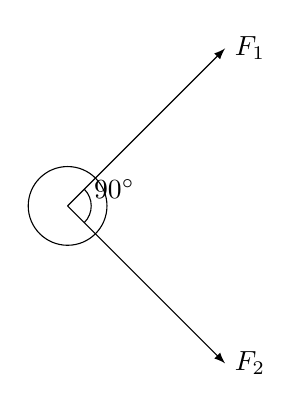
\begin{tikzpicture}[>=latex]
\draw (0,0) circle (.5cm);
\draw[->](0,0)--(2,2)node [right]{$F_1$};
\draw[->](0,0)--(2,-2)node [right]{$F_2$};
\draw (.3,0) arc (0:45:.3)node [right]{$90^\circ$}; 
\draw (.3,0) arc (0:-45:.3); 
\end{tikzpicture}
\caption{}
\end{minipage}
\begin{minipage}[t]{0.48\textwidth}
\centering
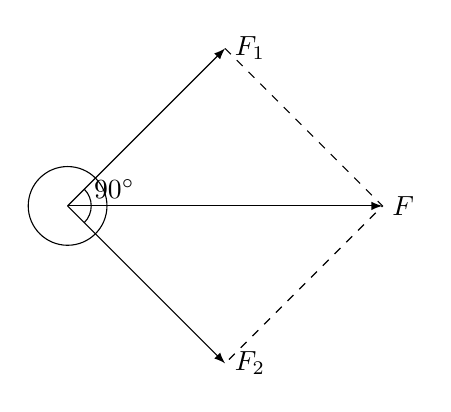
\begin{tikzpicture}[>=latex]
\draw (0,0) circle (.5cm);
\draw[->](0,0)--(2,2)node [right]{$F_1$};
\draw[->](0,0)--(2,-2)node [right]{$F_2$};
\draw (.3,0) arc (0:45:.3)node [right]{$90^\circ$}; 
\draw (.3,0) arc (0:-45:.3); 
\draw[->](0,0)--(4,0)node[right]{$F$};
\draw[dashed] (2,2)-- (4,0)--(2,-2);
\end{tikzpicture}
\caption{}
\end{minipage}
\end{figure}
    \end{solution}



\item 一个30牛的力水平地作用在2.0千克的物体上,使它在无摩擦的水平面上移动了3.0米的距离.然后,这个力变到15牛,又使物体移动了2.0米.物体增加的动能总共是多少?

\begin{solution}
    根据题意,$F_1=30$牛,$s_1=3.0$米,$F_2=15$牛,$s_2=
    2.0$米,则根据动能定理,物体增加的动能为:
 \[\begin{split}
     E_{k_2}-E_{k_1}=W=W_1+W_2&=F_1s_1+F_2s_2\\
    &=30\x3.0+15\x2.0\\
    &=120{\rm J}
 \end{split}\]
    
\end{solution}
\item 质量是2.0克的子弹,以300$\ms$的速度水平射入厚度是10毫米的钢板(图7.11),射穿后的速度是100$\ms$.子弹受到的平均阻力是多大?

\begin{figure}[htp]
    \centering
    \begin{tikzpicture}[>=latex, scale=1.4]
\draw [pattern=north east lines] (-.25,-1.5) rectangle (.25, 1.5);
\draw [|<->|] (-.25, 1.75)--node[above]{$s$} (.25,1.75);
\draw (-1, .1) --(-.6, .1) to [bend left=15] (-.45, 0) to [bend left=15] (-.6,-.1)--(-1,-.1)--(-1,.1); 

\node at (-.7, -.25){$m$};


\draw [dashed] (.5, .1) --(.9, .1) to [bend left=15] (1.05, 0) to [bend left=15] (.9,-.1)--(.5,-.1)--(.5,.1); 

\draw[->] (-1.3, .3)--node[above]{$v_1$}(-.4, .3);
\draw[->] (.4, .3)--node[above]{$v_2$}(1.1, .3);

\draw[->](.2,0)--node[above]{$f$}(-.2,0);

\end{tikzpicture}
    \caption{}
\end{figure}

\begin{solution}
已知$v_1=300\ms$,$v_2=100\ms$,$m=2.0\x10^{-3}{\rm kg}$,$s=10^{-2}{\rm m}$,根据动能定理
(考虑到阻力$f$做负功),
\[-fs=E_{k_2}-E_{k_1}\]
\[f=\frac{E_{k_1}-E_{k_2}}{s}=\frac{\frac{1}{2}m(v^2_1-v^2_2)}{s}=\frac{1.0\x 10^{-3}\x (300^2-100^2)}{2\x 10^{-2}}=8.0\x 10^3{\rm N}\]
子弹所受阻力为$8.0\x10^3$牛,方向与速度方向相反.
\end{solution}
\item 一架新型喷气式战斗机的质量是$1.50\times 10^4$千克,发动机的推力是$1.11\times 10^5$牛,起飞速度是88.0$\ms$,滑跑距离是671米.计算飞机起飞时受到的平均阻力.

\begin{solution}
    已知飞机质量$m=1.50\x10^4$千克,发动机推力$F=
    1.11\x10^5$牛,在起飞过程中,初速度$v_1=0$, 末速度就是起飞
    速度$v_2=88.0$米/秒,滑跑距离$s=671$米.在起飞时推力$F$
    和阻力$f$做功,根据动能定理,
\[Fs-fs=E_{k_2}-E_{k_1}=\frac{1}{2}mv^2_2\]
\[f=F-\frac{mv_2^2}{2s}=1.11\x 10^5-\frac{1.50\x 10^4\x (88.0)^2}{2\x 671}=2.44\x 10^4{\rm N}\]
\end{solution}
\end{enumerate}





\subsection{练习五}
下列各题中都以地面作参考平面.
\begin{enumerate}
    \item 体积相同的铝球和铅球,处在同一高度的地方,哪一
    个的重力势能较大?

    \begin{solution}
        铅球的重力势能大,因为铅球的质量大.
    \end{solution}
    \item 质量是2千克的物体位于0.8米高的桌面上,这个物体具有多少重力势能?
    \item 
    \begin{solution}
    \[E_p=mgh=2\x 9.8\x 0.8=15.7{\rm J}\]
    \end{solution}
    \item 图7.15是几个斜面,它们的高度相同,而倾角不同.
    让质量相同的物体沿斜面从顶端运动到底端,试根据功的公式来计算沿不同斜面重力所做的功,证明这个功跟斜面的倾角无关.
\begin{figure}[htp]
\centering \includegraphics[scale=1.3]{fig/7-15.pdf}
\caption{}
\end{figure}

\begin{solution}
    设三个斜面长度分别为$\ell_1$、$\ell_2$、$\ell_3$, 则物体沿第一个
    斜面从顶端运动到底端时,重力所做的功为:
  \[  W_1=mg\ell_1 \cos(90^{\circ}-\theta_1)=mg\ell_1\sin\theta_1=mgh\]
    同理,沿第二个斜面、第三个斜面运动到底端时,重力所
    做的功$W_2=W_3=mgh$, 与斜面的倾角无关.
\end{solution}
\item 图7.13表示一个斜抛物体的运动,当物体由抛出位置1运动到最高位置2时,重力所做的功是多少?物体克服重力所做的功是多少?由位置2运动到跟位置1在同一水平面上的位置3时,重力所做的功是多少?由位置1运动到位置3时,重力所做的功是多少?
\begin{figure}[htp]\centering
\begin{tikzpicture}[>=stealth, thick]
\fill [pattern = north east lines] (-1,-.25) rectangle (6,0);
\draw (-1,0)--(6,0);
\draw  (5,0) arc (0:180:2.5);
\draw [fill=gray!30] (0,.25) node {1} circle (.25) ;
\draw [dashed, fill=white] (5,.25) circle (.25) node  {3};
\draw [dashed] (2.5,2.5) circle (.25) node  [above] {2};
\draw [<->] (2.5,2.5)--node [fill=white]{$h$}(2.5,0);
\end{tikzpicture}
\caption{}
\end{figure}

\begin{solution}
    从位置1到位置2时,重力所做的功
\[    W_1=-mgh\]
    物体克服重力所做的功是$mgh$.

    从位置2到位置3时,重力所做的功$W_2=mgh$.

    从位置1到位置3时,重力所做的功$W_3=0$.
\end{solution}
\end{enumerate}


\subsection{练习六}
\begin{enumerate}
    \item 在下面列举的各个实例中,除(1)外都不计空气阻力,哪些机械能是守恒的?说明理由.
    \begin{enumerate}[(1)]
        \item 跳伞员带着张开的降落伞在空气中匀速下落.
        \item 抛出的手榴弹或标枪做斜抛运动.
        \item 用细绳拴着一个小球,绳的一端固定,使小球在光滑的水平面上做匀速圆周运动.
        \item 用细绳拴着一个小球,绳的一端固定,使小球在竖直平面上做圆周运动.
        \item 物体沿着光滑的曲面滑下(图7.14甲).
        \item 拉着一个物体沿着光滑的斜面匀速上升(图7.14乙).
        \item 在光滑水平面上运动的小球,碰到弹簧上,把弹簧压缩后又被弹簧弹回来(图7.14丙).
    \end{enumerate}
\begin{figure}[htp]
\centering\includegraphics[scale=.7]{fig/7-14.png}
\caption{}
\end{figure}

\begin{solution}
\begin{enumerate}
    \item 机械能不守恒.因为除重力外,降落伞还要克服
    空气阻力做功.
    \item 机械能守恒,因为除重力外,没有其他力对手榴弹或标枪做功.
    \item 机械能守恒,因为重力和支持力均不做功,细绳的拉
    力与位移始终垂直,也不做功.整个过程动能保持不变.
    \item 机械能守恒,因为除重力外,其他力(细绳拉力)不对
    物体做功.
    \item 机械能守恒,因为除重力外,曲面弹力始终与位移
    垂直,不做功.
    \item 机械能不守恒,因为除重力外,还有拉力对物体做功.
    \item 机械能守恒,因为除弹簧弹力外,没有其他力对小球
    做功.
\end{enumerate}
\end{solution}
    \item  做下面的实验,把物体拴在细线上悬挂起来,做成
    一个单摆(图7.15).把物体从平衡位置$O$拉到$B$,放手后观察物体的来回摆动,把铅笔放在位置1和2,可以看到物体仍然要升到跟$B$同样高的$C_1$和$C_2$.解释这个现象.
\begin{figure}[htp]
\centering
\begin{tikzpicture}[>=latex]
    \fill [pattern = north east lines] (-.5,0) rectangle (.5,0.2);
\draw (-.5,0)--(.5,0);
    \draw (0,0)--(0,-4);
    \draw (0,-.5) arc (-90:-45:.5)node[below]{$\theta$};
    \draw [dashed] (0,0)--(-45:4)--(-135:4)--(0,0);
    \draw[dashed] (0,-4) arc (-90:-45:4);
    \draw[dashed] (0,-4) arc (-90:-135:4);

    \draw[dashed] (0,-1) --(-2.2,-4/1.414);
\draw[dashed] (0,-2) --(-1.5,-4/1.414);
\draw[dashed] (-2.2,-4/1.414) to [bend right=25] (0,-4);
\draw[dashed] (-1.6,-4/1.414) to [bend right=30] (0,-4);

\draw[fill=black] (0,-1) circle (1.5pt)node[right]{1};
\draw[fill=black] (0,-2) circle (1.5pt)node[right]{2};

\draw [fill=white] (-45:4) circle (3pt)node[below]{$B$};
\draw [fill=white] (-135:4) circle (3pt)node[above]{$C$};
\draw [fill=white] (0,-4) circle (3pt)node[below]{$O$};
\draw [fill=white] (-2.2,-4/1.414) circle (3pt)node[above]{$C_1$};
\draw [fill=white] (-1.6,-4/1.414) circle (3pt)node[above]{$C_2$};

\draw [|<->|](.18,.18) to node [fill=white]{$\ell$} (2*1.414+.18, -2*1.414+.18) ;

\end{tikzpicture}
\caption{}
\end{figure}

\begin{solution}
    在单摆摆动过程中,除重力外,细绳对小球的拉力始
    终跟位移垂直,不做功,所以机械能守恒.当小球从$B$运动到
    $O$时,重力势能转化为动能.从$O$运动到$C$时,动能转化为重
    力势能,所以$C$与$B$等高.当铅笔在位置1和2阻挡摆线时,
铅笔作用在摆线的力对小球不做功,单摆机械能仍然守恒,当
小球摆到最高点$C_1$和$C_2$时,小球所具有的重力势能应与在
$B$、$C$处一样,所以$C_1$和$C_2$的位置也应与$B$和$C$等高.
\end{solution}
\end{enumerate}







\subsection{练习七}
\begin{enumerate}
    \item 滑雪运动员从25米高的山坡上滑下,如果阻力忽略不计,他滑到坡底时的速度是多大?

    \begin{solution}
        因为忽略阻力,所以滑下时只有重力做功,机械能守
        恒:
\[    mgh=\frac{1}{2}mv^2\]
      \[  v=\sqrt{2gh}=\sqrt{2\x9.8\x25}=22.1\ms\]
    \end{solution}
    \item 物体从高的光滑斜面的顶端滑下,证明物体到达斜面末端时的速度 $v=\sqrt{2gH}$.

    \begin{proof}
        物体从光滑斜面滑下,机械能守恒,所以
        \[mgH=\frac{1}{2}mv^2,\qquad v=\sqrt{2gH}\]
    \end{proof}
    \item 蒸汽打桩机的重锤的质量是250千克,把它提升到离地面25米高处,然后让它自由落下.计算:
    \begin{enumerate}
        \item 重锤在最高点的动能、重力势能和机械能.
        \item 重锤下落10米时的重力势能、动能和速度.
        \item 重锤落到地面时的重力势能、动能和速度.
    \end{enumerate}

    \begin{solution}
\begin{enumerate}
    \item 重锤在最高点时的动能$E_k=0$, 重力势能$E_p=
    mgh=250\x9.8\x25=6.13\x10^4{\rm J}$.机械能$E=E_k+E_p=
    6.13\x10^4{\rm J}$.
    \item 重锤下落10米时,其高度$h'=15$米,重力势能$E'_p=
    mgh'=250\x9.8\x15=3.68\x10^4{\rm J}$.由于机械能守恒,则
    动能
    \[E'_k=E-E'_p=6.13\x10^4-3.68\x10^4=2.45\x10^4{\rm J}\]
    因为$E'_k=\frac{1}{2}m{v'}^2$, 所以
\[v'=\sqrt{\frac{2E_k'}{m}}=\sqrt{\frac{2\x 2.45\x 10^4}{250}}=14\ms\]
    \item 重锤落到地面时,$h''=0$, 所以$E''_p=0$.
    $E''_k=E=6.13\x10^4{\rm J}$
    \[v''=\sqrt{\frac{2E_k''}{m}}=\sqrt{\frac{2\x 6.13\x 10^4}{250}}=22.1\ms\]
\end{enumerate}
    \end{solution}
\item 要使一球着地后回跳的高度超过原高10米,必须以多大速度将它下抛?不计球击地时的能量损失.

\begin{solution}
    设原高为$h$, 则根据机械能守恒定律
   \[\begin{split}
       mgh+\frac{1}{2}mv^2&=mg(h+10{\rm m})\\
\frac{1}{2}mv^2&=mg\x 10{\rm m}\\
v&=\sqrt{2g\x 10{\rm m}}=\sqrt{2\x 9.8\x 10}\ms=14\ms
   \end{split} \]
    为使一球着地后回跳高度超过原高10米,必须以14$\ms$的初速度下抛.
\end{solution}
\item 一个物体从距地面40米的高处自由落下,经过几秒后,该物体的动能和重力势能相等?$g=10\msq$.

\begin{solution}
    已知高度$H=40$米,设在$h$高度时物体的运动速
    度为$v$, 动能和势能相等,则
    \[\frac{1}{2}mv^2=mgh\]

    根据机械能守恒定律,又有$mgh+\frac{1}{2}mv^2=mgH$(图
7.16),两式中消去$\frac{1}{2}mv^2$,得
\[2mgh=mgH,\qquad h=\frac{H}{2}=20{\rm m}\]

说明到动能和重力势能相等时,已
落下距离$h'$也是20米.因为是自由落
体,所以
\[h'=\frac{1}{2}gt^2,\qquad t=\sqrt{\frac{2h'}{g}}=\sqrt{\frac{2\x 20}{10}}=2{\rm s}\]
\end{solution}
\end{enumerate}

\begin{figure}[htp]
    \centering
\begin{tikzpicture}[>=latex]
\draw(-1,0)--(1,0);
\fill[pattern=north east lines](-1,-.2) rectangle (1,0);
\draw[<->](0,0)--node[fill=white]{$h$}(0,2);
\draw[<->](0,2)--node[fill=white]{$h'$}(0,3.5);
\draw[<->](.5,0)--node[fill=white]{$H$}(.5,3.5);
\draw(-.5,2.2) circle(.2);
\draw(-.5,3.7) circle(.2);
\draw[->](-1,2.4+.1)--node[left]{$v$}(-1,2-.1);
\draw(-.2,3.5)--(.8,3.5);
\draw(-.2,2)--(.2,2);
\end{tikzpicture}
    \caption{}
\end{figure}


\subsection{习题}
\begin{enumerate}
    \item 一个原来静止的物体,在力$F$的作用下,沿着力的方向移动一段距离$s$,得到速度$v$.如果移动的距离不变,力$F$增大到$n$倍,得到的速度也增大到$n$倍.这话对吗?速度应该增大到多少倍?

    \begin{solution}
        不对,力$F$增大到$n$倍时,功$W=Fs$增大到原来的
        $n$倍,由于物体初始是静止的,所以根据动能定理,物体得到
        的动能为原来的$n$倍,即
        \[E'_k=nE_k,\qquad \frac{1}{2}m(v')^2=\frac{n}{2}mv^2,\qquad v'=\sqrt{n}\cdot v\]
  所以速度应增大到$\sqrt{n}$倍,而不是$n$倍.
    \end{solution}
    \item 在水平面上有两个质量不同而具有相同动能的物
体,它们所受的阻力相等.这两个物体停止前经过的距离是否相同?停下来所用的时间是否相同?

\begin{solution}
由于两个物体动能相同,使物体停止下来,动能变化
相等.根据动能定理,
\[-fs=0-E_k=-E_k\]
阻力所做的功应
相等.又因为阻力$f$相等,所以位移$s$也应相同.

停止下来所用的时间$t$可用匀减速运动的速度公式来讨
论:
\[0=v_0-at,\qquad t=\frac{v_0}{a}\]
根据动能的定义式,
\[v_0=\sqrt{\frac{2E_k}{m}}\]
根据牛顿第二定律$a=f/m$,
把$v_0$和$a$代入前式求$t$, 得
\[t=\frac{\sqrt{\dfrac{2E_k}{m}}}{\dfrac{f}{m}}=\frac{\sqrt{2E_k\cdot m}}{f}\]
因为两个物体的$E_k$相同,$f$相同,而$m$不同,所以时间$t$也不
相同.
\end{solution}
\item 质量是$m$千克的物体自由落下,在第1秒内和第2秒内物体重力势能的减少各是多少?

\begin{solution}
重力势能的减少等于重力所做的功$W$, 而$W=mgh$, 
自由落体在第1秒和第2秒内下落的距离分别为$h_1$和$h_2$
\[\begin{split}
    h_1&=\frac{1}{2}gt_1^2=4.9{\rm m}\\
    h_2&=\frac{1}{2}gt_2^2-\frac{1}{2}gt_1^2=19.6-4.9=14.7{\rm m}
\end{split}\]
所以,物体在第1秒内减少的重力势能
\[W_1=mgh_1=m\x9.8\x4.9=43m{\rm J}\]
物体在第2秒内减少的重力势能
\[W_2=mgh_2=m\x9.8\x14.7=144m{\rm J}\]
\end{solution}
\item 从地面竖直上抛一个物体,质量是0.2千克,经过8秒落回原地.物体抛出时的动能是多少?从被抛出到最高点,物体克服重力所做的功是多少?物体上升到最高点时的重力势能是多少?不计空气阻力.

\begin{solution}
上抛物体经过8秒落回原地,则上抛和下落时间均
为4秒.上抛高度
\[h=\frac{1}{2}gt^2=\frac{1}{2}\x 9.8\x 4^2=78.4{\rm m}\]
根据机械能守恒定律,抛出时的动能等于最高点时的重
力势能,所以
\[E_k=E_p=mgh=0.2\x9.8\x78.4=154{\rm J}\]

从抛出点到最高点,物体克服重力所做的功等于重力势
能的增加,为154焦.

物体上升到最高点时的重力势能也是154焦.
\end{solution}
\item 一个人站在10米高的楼上沿斜上方抛出一个小球,初速度的大小是10$\ms$,抛出角是30$^\circ$.小球落地时速度是多大?如果初速度的大小不变,沿斜下方抛出小球,抛射角是45$^\circ$,小球落地时速度是多大?用其他某个角度抛出,结果又怎
样?不计空气阻力.

\begin{solution}
小球在运动过程中,除重力以外,没有其他力做功,
所以机械能守恒.
\[\frac{1}{2}mv_0^2+mgh=\frac{1}{2}mv^2\]
\[v=\sqrt{v^2_0+2gh}=\sqrt{10^2+2\x9.8\x10}=17.2\ms\]

只要抛出时的速度大小不变,高度不变,则落地时速度大
小$v=\sqrt{v^2_0+2gh}$也不变,与抛出时速度的方向无关.
\end{solution}
\item 利用机械能守恒定律,你能算出平抛和斜抛物体通过任意位置时速度的大小吗?怎样计算?

\begin{solution}
设平抛和斜抛物体的抛出点离地面高$h_0$, 抛出时的
速度大小为$v_0$, 则根据机械能守恒定律:
\[\frac{1}{2}mv_0^2+mgh_0=\frac{1}{2}mv^2+mgh\]
式中$v,h$分别为任一时刻的速度大小和高度,经整理后,可
得出
\[v=\sqrt{v^2_0+2g(h_0-h)}\]
利用这个式子可以求出物体通过任意位置(高度)的速度
大小.
\end{solution}
\item 质量是0.25千克的球以2.0$\ms$的速度向右运动,然后沿着图7.17所示的光滑的凹面滚动,这个小球在凹面的右侧能滚上多高?如果在$P$点把球从静止放开,它能滚上多高?
\begin{figure}[htp]\centering
\includegraphics[scale=.7]{fig/7-17.png}
\caption{}
\end{figure}

\begin{solution}
设小球在凹面右侧能滚上的高度为$h$, 在小球运动
过程中,除重力外,没有其他力做功,所以机械能守恒.
\[\frac{1}{2}mv^2_0+mgh_0=mgh\]
式中$v_0$为初速度,$h_0$为初始高度,由上式可得
\[h=\frac{v^2_0}{2g}+h_0=\frac{2.0^2}{2\x 9.8}+1=1.2{\rm m}\]
如果小球从$P$点由静止开始运动,则能滚上的高度应同
$P$点相同,即0.5米.
\end{solution}
\item  一颗子弹以700$\ms$的速度打穿第一块木板后,这度减低到500$\ms$.如果让它继续打穿第二块同样的木板,它的速度将变为多大?它能否再打穿第三块同样的木板?

\begin{solution}
设子弹每穿过一块木板,克服阻力所做的功是一样
的,子弹动能的减少也是相同的.根据题意,子弹的初动能
\[E_{k_2}=\frac{1}{2}mv^2_0=\frac{1}{2}m\x(700\ms)^2=2.45\x10^5m {\rm m^2/s^2}\]
穿过第一块木块后的动能
\[E_{k_1}=\frac{1}{2}mv^2_1=\frac{1}{2}m\x(500\ms)^2=1.25\x10^5m {\rm m^2/s^2}\]
子弹每穿过一块木板动能的减少为
\[\begin{split}
    \Delta E_k&=\frac{1}{2}mv^2_0-\frac{1}{2}mv^2_1\\
&=2.45\x10^5m - 1.25\x10^5m\\
&=1.20\x 10^5m {\rm m^2/s^2}
\end{split}\]
子弹穿过第二块木板后的动能为
\[E_{k_2}=E_{k_1}-\Delta E_k=1.25\x10^5m -1.20\x10^5m
=0.5\x10^4m {\rm m^2/s^2}\]
速度为
\[v_2=\sqrt{\frac{2E_{k_2}}{m}}=\sqrt{2\x 0.5\x 10^4}=100\ms\]

由于$E_{k_2}<\Delta E_k$, 所以子弹不能再穿过第三块木板.
\end{solution}
\item  列车经过一段长2.1千米的平直铁路,速度从54$\kmh$增加到72$\kmh$,列车重1400吨,列车受到的阻
是车重的$k=0.003$倍.求机车的功率.

\begin{solution}
已知列车的初速$v_1=54\kmh=15\ms$,末
速$v_2=-72\kmh=20\ms$.列车质量$m=1400{\rm t}=
1.4\x10^6{\rm kg}$,阻力
\[f=kmg=0.003\x9.8\x1.4\x10^6=4.12\x10^4{\rm N}\]
火车的位移$s=2.1\x10^3$米.

设牵引力$F$对列车做功为$W_{\text{牵}}$.根据动能定理,
\[W_{\text{牵}}-fs-\frac{1}{2}mv^2_2-\frac{1}{2}mv_1^2\]
所以
\[\begin{split}
    W_{\text{牵}}&=fs+\frac{1}{2}mv^2_2-\frac{1}{2}mv^2_1\\
&=4.12\x10^4\x2.1\x10^3+\frac{1}{2}\x 1.4\x 10^6\x 20^2-\frac{1}{2}\x1.4\x10^6x20^2-\frac{1}{2}\x1.4\x10^6\x15^2\\
&=2.09\x10^8{\rm J}
\end{split}\]

整个加速过程所花的时间$t$可以通过匀变速运动的规律
求出.由$s=vt=\dfrac{v_1+v_2}{2}t$得
\[t=\frac{2s}{v_2+v_1}=\frac{2\x 2.1\x 10^3}{20+15}=120{\rm s}\]
所以列车牵引力的功率
\[P=\frac{W_{\text{牵}}}{t}=\frac{2.09\x 10^{8}}{120}=1.74\x 10^6{\rm W}\]

说明:这一题还可以先通过动能定理求牵引力$F$, 再根据$\bar v=\dfrac{v_1+v_2}{2}$.求出列车平均速度.然后根据$P=F\bar v$求得功率.
\end{solution}
\item  在一个农村小水电站里,上下游的水位差是3米,每秒钟有0.5${\rm m^3}$的水流过发电机的水轮机,从水轮机流出的水的速度是3$\ms$,上游水的流速忽略不计.设水流能的70\%可以转化成电能,求这个小水电站发出的电功率.

\begin{solution}
    算出1秒钟内所产生的电能,叩能得到电功率.
    $0.5{\rm m^3}$的水的质量
\[m=\rho V=1\x 10^3\x 0.5=500{\rm kg}\]
\[\begin{split}
P&=\frac{E_{\text{电}}}{t}=\frac{(E_p-E_k)\x 70\%}{t}\\
&=\frac{(mgh-\frac{1}{2}mv^2)\x 70\%}{t}\\
&=\frac{(500\x 9.8\x 3-\frac{1}{2}\x 500\x 3^2)\x 70\%}{1}=8.7{\rm kW}
\end{split}\]
\end{solution}
\item  飞机、轮船所受的空气或水的阻力并不是固定的,它跟飞机、轮船的速度有关.当速度很大时,阻力与速度的平方成正比,试证明:这时要把飞机、轮船的最大速度增大到2倍,发动机的额定功率要增大到8倍才行.这就是在增大飞机、轮船等交通工具的速度方面,每取得一个新的成就都很不容易的原因.

\begin{solution}
    因为阻力$f$与速度的平方成正比,即$f\propto v^2$, 所以,
    当$v$增大为原来的2倍时,$f$增为原来的4倍,此时,为使飞机、
    轮船能继续以这么大的速度前进,牵引力$F$至少等于 $f$, 也应
    增为原来的4倍.由公式$P=Fv$可知,当$v$增加原来的2倍
    时,$F$增为原来的4倍,则额定功率$P$应增为原来的8倍.
\end{solution}
\item 一辆汽车沿着平直的道路行驶,遇有紧急情况而刹车,刹车后轮子只滑动不滚动,从刹车开始到汽车停下来,汽车前进12米.已知轮胎与路面之间的滑动摩擦系数$\mu=0.7$.求刹车前汽车的行驶速度,不计空气阻力.

\begin{solution}
    汽车刹车后,在水平方向上只受阻力$f$的作用前进
    $s=12$米,设汽车质量为$m$, 则$f=\mu N=\mu mg$.

    根据动能定理,有
    \[-fs=0-\frac{1}{2}mv^2_1\]
    则
    \[\mu mgs=\frac{1}{2}mv^2_1\]
    所以
   \[ v_1=\sqrt{2\mu gs}=\sqrt{2\x0.7\x9.8\x12}=12.8\ms\]
\end{solution}
\item 一辆5吨的载重汽车开上一个坡路,坡路长$s=100$米,坡顶和坡底的高度差$h=10$米,汽车上坡前的速度是10$\ms$,上到坡顶时减为5.0$\ms$.汽车受到的摩擦阻力是车重的$k=0.05$倍.求汽车的牵引力.取$g=10\msq$.

\begin{solution}
    汽车在上坡过程中,牵引力做功为$Fs$, 克服重力做
    的功为$mgh$, 克服阻力做的功为$kmgs$. 根据动能定理,
\[    Fs-mgh-kmgs=\frac{1}{2}mv^2_2-\frac{1}{2}mv^2_1\]
\[\begin{split}
    F&=\frac{mgh+kmgs+\frac{1}{2}mv^2_2-\frac{1}{2}mv^2_1}{s}\\
    &=\frac{5\x10^3\x10\x10+0.05\x5\x10^3\x10\x100
    +\frac{1}{2}\x5\x10^3\x5.0^2-\frac{1}{2}
    \x5\x10^3\x10^2}{100}\\
&=5.6\x10^3{\rm N}
\end{split}\]
    说明:在这个题目里,汽车牵引力做的功:
\[W_1=Fs=5.6\x 10^3\x 100=5.6\x 10^5{\rm J}\]
汽车增加的机械能:
\[\begin{split}
    E_2-E_1&=\frac{1}{2}mv^2_2+mgh-\frac{1}{2}mv^2_1\\
    &=\frac{1}{2}\x 5\x 10^3\x 5.0^2+5\x 10^3\x 10\x 10-\frac{1}{2}\x 5\x 10^3\x 10^2\\
    &=3.1\x 10^5{\rm J}
\end{split}\]
其中增加的动能为
\[\begin{split}
    E_{k_2}-E_{k_1}&=\frac{1}{2}mv^2_2-\frac{1}{2}mv^2_1\\
    &=\frac{1}{2}\x 5\x 10^3\x 5.0^2-\frac{1}{2}\x5\x10^3\x10^2\\
    &=-1.9\x10^5{\rm J}
\end{split}\]
说明动能是减少了$1.9\x10^5$焦.

增加的重力势能是
\[mgh=5\x10^3\x10\x10=5\x10^5{\rm J}\]
克服摩擦力做功是:
\[fs=kmgs=0.05\x5\x10^3\x10\x100=2.5\x10^5{\rm J}\]

这一题前面是用动能定理求解的,现在经过分项计算,可
以进一步看出,汽车牵引力所做的功除一部分来克服阻力
做功外,其余的全部转化为机械能.
\end{solution}
\item 一个滑雪的人从高度为$h$的斜坡上由静止开始滑下,然后在水平面滑行一段距离停下来(图7.18).已知斜面的倾角为$\theta$,滑雪板和雪之间的滑动摩擦系数为$\mu$,求滑雪人在水平面上滑行的距离$s_1$.你能不能求出滑雪人通过的水
平距离$s$?其他条件不变,只改变斜坡的倾角$\theta$,水平距离$s$是否改变?为什么?
\begin{figure}[htp]\centering
    \begin{tikzpicture}[>=stealth]
\fill [pattern = north east lines, rotate=-30] (0,-.25) rectangle (4,0);
\draw [rotate=-30](0,0)--(4,0);
\fill [pattern = north east lines] (3.45,-2) rectangle (5.5,-2-.25);
\draw (3.45,-2)--(5.5,-2);

\draw[|<->|] (3.45,-2.5)--node[fill=white]{$s_1$}(5.5,-2.5);
\draw[|<->|] (0,-2.75)--node[fill=white]{$s$}(5.5,-2.75);
\draw[|<->|] (0,0)--node[fill=white]{$h$}(0,-2);
\draw[dashed] (-0.5,-2)--(3.45,-2);
\draw[dashed] (0,-2)--(0,-2.75);
\draw[dashed] (5.5,-2.75)--(5.5,-2.25);
\draw  (3.45-1,-2+.55) node[below] {$\theta$}  arc (145:180:1);
    \end{tikzpicture}
    \caption{}
\end{figure}


\begin{solution}
    设斜坡长为$\ell$, 人滑至斜面底端时的速度为$v$. 在下
    滑过程中,重力做功为$mgh$, 摩擦力做功为
\[-\mu mg\ell \cos\theta=-\mu mg\cos\theta\cdot \frac{h}{\sin\theta}=-\mu\frac{mgh}{\tan\theta}\]

根据动能定理:
\begin{equation}
    mgh-\frac{\mu mgh}{\tan\theta}=\frac{1}{2}mv^2
\end{equation}
在水平面上滑行阶段,只有摩擦力做功,则根据动能定理
可得.
\begin{equation}
    -\mu mgs_1=-\frac{1}{2}mv^2
\end{equation}
(7.1)式和(7.2)式相加,消去$\frac{1}{2}mv^2$,得
\[mgh-\frac{mu mgh}{\tan\theta}-\mu mgs_1=0\]
解得:\[s_1=\frac{h}{\mu}-\frac{h}{\tan\theta}\]
又因为$s-s_1=\dfrac{h}{\tan\theta}$,所以
\[s=s_1+\frac{h}{\tan\theta}=\frac{h}{\mu}-\frac{h}{\tan\theta}+\frac{h}{\tan\theta}=\frac{h}{\mu}\]
可见,$s$与角度$\theta$无关,所以若改变斜坡倾角$\theta$, 水平距离$s$将
不改变.

说明:这一题如果把斜面和平面上的运动看作是一个运
动过程,也可以同样应用动能定理.但此时摩擦力做功要分
两段计算后相加.因为在这两个阶段中,摩擦力的大小是不
同的,全过程的动能定理形式应为:
\[mgh-\frac{mu mgh}{\tan\theta}-\mu mgs_1=0\]
与前一种解法中消去
$\frac{1}{2}mv^2$后的式子一样,但对一般同学来
说,还是分段应用动能定理为好.
\end{solution}
\item 要使小球滑到光滑的离心轨道顶端时不落下来(图7.25),至少应使它在斜轨上多高处由静止开始下滑?


\begin{figure}[htp]\centering
    \begin{tikzpicture}[>=stealth, scale=1.2]
\draw (-1,0)--(6,0);
\fill [pattern = north east lines] (-1,-.25) rectangle (6,0);

\draw (0,1) circle(1);
\draw (.275,0)--(5,3);
\draw [|<->|](5,0)--node [fill=white]{$h$}(5,3)node[above]{$m$};
\draw [fill=gray](4.6,3) circle (.2);
\draw [dotted](0,2-.2) circle (.2);

\draw[->](0,1)--node [fill=white]{$R$}+(30:1);
\draw [->](0,2-.2)--(.5,2-.2)node[below]{$v$};
\fill (0,1) circle(1pt);
\fill (0,2-.2) circle(1pt);
    \end{tikzpicture}
    \caption{}
\end{figure}


\begin{solution}
    设小球运动到圆形轨道顶端而不落下来的最小速度为$v$, 此时小球已不受圆形轨道的作用而仅靠重力提供向心
    力.因此
    \begin{equation}
        mg=\frac{mv^2}{R}
    \end{equation}

    考虑到小球在整个运动过程中除重力外其他力均不做
    功,所以机械能守恒,则
\begin{equation}
    mgh=mg(2R)+\frac{1}{2}mv^2
\end{equation}
将(7.3)式代入(7.4)式,消去$v^2$, 得
\[mgh=2mgR+\frac{1}{2}mgR=\frac{5}{2}mgR\]
解得:
\[h=\frac{5}{2}R\]
\end{solution}
\end{enumerate}


\section{参考资料}
\subsection{关于系统的动能定理}
课本得到的动能定理$W=E_{k_2}-E_{k_1}$,是以一个物体为研
究对象的,式中$W$为所有外力(包括重力、弹力)所做的功.这
一定理可推广到由几个物体构成的物体系中去.但定理的形
式应作相应的变动.因为对一个物体系来说,在状态变化过
程中,不仅有外力做功,还有可能有内力作功.内力作功也会
改变整个系统的总动能,例如系统内的爆炸力做功(如手榴
弹爆炸)可使整个系统的动能增加;系统内的摩擦力作功又可
以使整个系统的动能减少.爆炸力和摩擦力都不是保守力,
它们所做的功可以写成$W_{\text{非保守}}$.此外,跟中学课本不同,在普通物理中一般把重力和弹力也看作是系统的内力(把地球和
弹簧等都包括在系统之中),它们所做的功可写成$W_{\text{保守}}$. 这
样,系统的动能定理可以写成:
\[W_{\text{外力}}+W_{\text{保守}}+W_{\text{非保守}}=E_{k_2}-E_{k_1}\]

在系统的动能定理中,因为保守内力(重力和弹力)所做
的功等于相应势能增量的负值,即
\[W_{\text{保守}}=-\Delta E_p=E_{p_1}-E_{p_2}\]
代入系统的动能定理并移项,得
\[W_{\text{外力}}+W_{\text{非保守}}=E_{k_2}-E_{k_1}+E_{p_2}-E_{p_1}=(E_{k_2}+E_{p_2})-(E_{k_1}+E_{p_1})\]
如果$W_{\text{外力}}=0$,$W_{\text{非保守}}=0$,则
\[(E_{k_2}+E_{p_2})-(E_{k_1}+E_{p_1})=0\]
系统的机械能守
恒,所以严格讲,机械能守恒的条件是系统外力不做功,非保
守内力也不做功.

